\documentclass{beamer}
%\usetheme{Ilmenau}
%\usecolortheme{beaver}

\usepackage[slovak,american]{babel}
\usepackage[utf8]{inputenc}
\usepackage{graphicx}
\usepackage{adjustbox}
 \usepackage{xcolor}
 
 \newsavebox\MBox
\newcommand\Cline[2][red]{{\sbox\MBox{$#2$}%
  \rlap{\usebox\MBox}\color{#1}\rule[-2.2\dp\MBox]{\wd\MBox}{1pt}}}

%\usefonttheme{serif}

\definecolor{UKOrange}{HTML}{ef9424} %
\definecolor{UKBrown}{HTML}{a96d5e} %
\definecolor{UKLight}{HTML}{d8b6ab} %
\definecolor{UKDark}{HTML}{7a4f44}
\definecolor{UKDarker}{HTML}{4d312b} 
\definecolor{UKDarkest}{HTML}{2e1e1a}
\definecolor{UKRed}{HTML}{bf1f1c}

\setbeamertemplate{footline}[frame number]{}
\setbeamertemplate{navigation symbols}{}

%\usecolortheme{beaver}
\setbeamertemplate{itemize item}[square]
\setbeamercolor{itemize item}{fg = UKBrown}
\setbeamercolor{itemize subitem}{fg = UKLight}
\setbeamercolor{enumerate item}{fg = UKDark}

\setbeamercolor{footnote}{fg=UKLight}
\setbeamercolor{footnote mark}{fg=UKLight}
\setbeamerfont{footnote}{size=\tiny}
\renewcommand\footnoterule{}

\usetheme{default}
\beamertemplatenavigationsymbolsempty
\setbeamercolor{title}{fg=white, bg=UKBrown}
\setbeamercolor{frametitle}{fg=white, bg=UKBrown}
\setbeamercolor{block title}{bg=UKBrown, fg= white}
\setbeamercolor{block body}{bg =UKLight, fg = UKDarkest}

\useoutertheme[subsection=false]{miniframes}
\AtBeginSection[]{\subsection{}}

\setbeamercolor{below lower separation line head}{bg=UKDark}
\addtobeamertemplate{headline}{}{%
  \begin{beamercolorbox}[colsep=0.5pt]{below lower separation line head}
  \end{beamercolorbox}
}
%\setbeamercolor*{mini frame}{fg=white,bg=UKRosy}
\setbeamercolor{section in head/foot}{fg=UKLight, bg=UKDark}

%\setbeamertemplate{itemize/enumerate body begin}{\normalsize}
%\setbeamertemplate{itemize/enumerate subbody begin}{\normalsize}




%\newcommand{\codeblock}[2]{ \begin{block}{#1} \begin{verbatim}#2\end{verbatim}\end{block}}

%\defbeamertemplate*{title page}{customized}[1][]
%{
%  \begin{centering}
%    \begin{beamercolorbox}[sep=8pt,center]{title}
%      \usebeamerfont{title}\inserttitle
%    \end{beamercolorbox}
%  \end{centering}
%  \bigskip
%
%\begin{columns}[onlytextwidth,T]
%
%
%  \column{27mm}
%  \includegraphics[width=27mm]{images/logoFMFI.png}
%  
%  \column{\dimexpr\linewidth-54mm-6mm}
%  \centering
%  \vspace{5mm}  
%  \usebeamerfont{author}\insertauthor\par
%  \vspace{5mm}
%  \usebeamerfont{institute}\insertinstitute\par
%
%  \column{27mm}
%  \includegraphics[width=27mm]{images/logoUK.png}  
%\end{columns}
%\centering
%\vspace{7mm}
%  \usebeamerfont{date}\insertdate\par
%}


\title[kNN]{Rozpoznávanie obrazcov - 7 cvičenie \\ kNN a validácia}
\author[Viktor Kocur]{Viktor Kocur \\{\small viktor.kocur@fmph.uniba.sk}}
\institute{DAI FMFI UK}
\date{6.4.2020}
%\titlegraphic{\includegraphics[width=2.7cm]{images/logoFMFI.png}\hspace*{1cm}~%
%   \includegraphics[width=2.7cm]{images/logoUK.png}
%}


\begin{document}
\selectlanguage{slovak}

\begin{frame}[plain]
  \titlepage  
\end{frame}

\section{k nearest neighbors}

\begin{frame}
\frametitle{k nearest neighbors}
\begin{block}{Základný princíp}
Na príznakovom priestore $\mathbb{R}^n$ opatreným metrikou $\rho$ určíme triedu pre príznakový vektor $\vec{x} \in \mathbb{R}^n$ tak, že nájdeme $k$ prvkov z trénovacej množiny, ktoré sú k $\vec{x}$ najbližšie a triedu priradíme podľa toho ktorá trieda má najviac zástupcov z pomedzi $k$ susedov.
\end{block}

\begin{block}{Trénovanie?}
Táto metóda nevyžaduje trénovanie, vždy sa pozeráme na celú trénovaciu množinu a hľadáme tam susedov. Táto metóda je teda pomalá.
\end{block}
\end{frame}


\begin{frame}
\frametitle{Metriky}
\begin{block}{Definícia}
Majme množinu $P$. Potom metrika je funkcia $\rho: P \times P \mapsto \mathbb{R}_0^+$ taká že pre $\forall p, q, r \in P$ platí: \\
1. $\rho(p,q) \ge 0$ \\
2. $\rho(p,q) = 0 \Leftrightarrow p = q$ \\
3. $\rho(p,q) = \rho(q,p)$ \\
4. $\rho(p,r) \leq \rho(p,q) + \rho(q,r)$
\vspace{1em}
\\
Množinu s metrikou nazývame metrický priestor.
\end{block}
\end{frame}


\begin{frame}
\frametitle{Metriky}
\begin{block}{Metriky na $\mathbb{R}^n$}
$$\rho_e(\vec{x}, \vec{y}) = \sqrt{\sum_{i = 1}^n (x_i - y_i)^2 }   $$
$$\rho_m(\vec{x}, \vec{y}) = \sum_{i = 1}^n |x_i - y_i |   $$
$$\rho_q(\vec{x}, \vec{y}) = \left( \sum_{i = 1}^n (x_i - y_i)^q  \right)^{\frac{1}{q}} $$
$$\rho_{max}(\vec{x}, \vec{y}) = max_{i} | x_i - y_i |  $$
\end{block}
\end{frame}


\begin{frame}
\frametitle{Voľba k}
\center
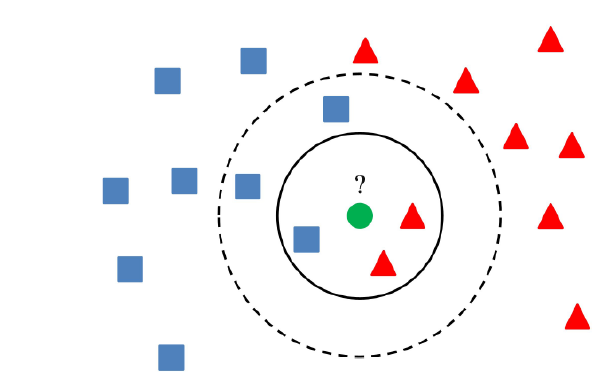
\includegraphics[width=0.8\textwidth]{knn2.png}
\end{frame}

\begin{frame}
\frametitle{Voľba k}
\center
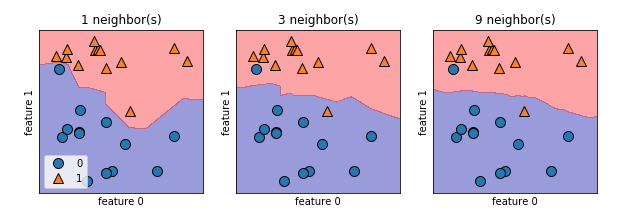
\includegraphics[width=1.1\textwidth]{knn.png}
\end{frame}


\begin{frame}
\frametitle{Úloha}
\begin{block}{Úloha}
Vytvorte vlastnú funkciu mykNN(k, X, y, p) - ktorá vráti triedu podľa k-NN na trénovacích dátach X s triedami y pre vektor p. 
\end{block}

\begin{block}{Úloha}
Funkciu otestujte na dátach z minulého cvičenia a fisheriris.
\end{block}
\end{frame}

\begin{frame}
\frametitle{Úloha}
\begin{block}{fitcknn}
Mdl = fitcknn(X,y) - vytvorí knn klasifikátor podobne ako na minulom cvičení 
\end{block}

\begin{block}{predict}
Mdl.predict(x) - vráti predpoveď modelu
\end{block}

\begin{block}{Properties}
Zaujímavé properties sú: 'Standardize', 'Distance', 'NumNeighbors', 'NSMethod'. Pozrite si ich v helpe.
\end{block}

\begin{block}{Úloha}
Upravte m-file na zobrazovanie hraníc SVM klasifikátora z minulého cvičenia a zobrazte si hranice pre kNN.
\end{block}
\end{frame}


\section{Validácia}
\begin{frame}
\frametitle{Rozdelenie dát}
\begin{block}{Trénovacia množina}
Doteraz sme vždy operovali s trénovacou množinou. Teda všetky dáta sme použili na nastavenie parametrov modelu.
\end{block}

\begin{block}{Testovacia množina}
V prípade, že chceme overiť že náš model je spoľahlivý je nutné odložiť si časť dát na testovanie. Testovacie dáta použijeme až na úplnom konci keď máme model hotový. Používame ich čisto na vyhodnotenie a nie na určenie metódy, alebo parametrov a hyperparametrov modelu.
\end{block}
\end{frame}


\begin{frame}
\frametitle{Rozdelenie dát}
\begin{block}{Validačná množina}
Keďže testovaciu množinu nepoužívame na určenie modelu, tak potrebujeme ešte jednu množinu na tento účel. Validačnú množinu používame na určenie správneho prístupu a nastavenie hyperparametrov modelu. 
\end{block}

\begin{block}{Rozdelenie dát}
Podiely na rozdelovanie dát záležia od ich charakteru, množstva a modelu. Pri neurónových sieťach potrebujeme veľa trénovacích dát, preto je vhodné využiť split 80/10/10. Pri metódach aké sme si zatiaľ ukázali stačí aj 60/20/20. V niektorých prípadoch však je nutné isť ešte ďalej. Existujú datasety kde je split napr. 40/20/40.
\end{block}
\end{frame}


\begin{frame}
\frametitle{Validácia - postup}
\begin{block}{Hyperparametre}
Na validačnej množine určujeme hyperparametre. To sú parametre/nastavenia, ktoré menia spôsob akým sa model trénuje a ako funguje predikcia. Pre SVM je to napr. výber kernelovej funkcie a jej škály. Pre kNN je to napríklad hodnota $k$ a výber metriky. 
\end{block}

\begin{block}{Validácia}
Pre rôzne hyperparametre natrénujeme (v prípade kNN len vytvoríme) na trénovacej množine naše modely. Tieto potom otestujeme na validačnej množine.  Použijeme na to nejakú mieru spoľahlivosti. Ideálne presnosť klasifikácie. Na základe výsledkov vyberieme hyperparametre.
\end{block}
\end{frame}



\begin{frame}
\frametitle{Validácia - úloha}
\begin{block}{Úloha}
Rozdelte si dáta z predchádzajúceho cvičenia na train/val/test s pomerom 60/20/20. A určite najlepší parameter $k$ pre kNN klasifikátor a metriku na validačnej množine.
\end{block}

\begin{block}{Pozor na dostatočnú reprezentáciu}
Často sú dáta zoradené podľa triedy, alebo v nejajek inej pravidelnej forme. Je preto nutné overiť si, či je rozdelenie na train/val/test zmysluplné. Ideálne chceme rovnaký podiel tried pre každú množinu. 
\end{block}
\end{frame}

\begin{frame}[fragile]
\frametitle{Vzájomná validácia}
\begin{block}{Vzájomná validácia}
Ak máme málo dát tak nedelíme dáta na trénovacie a validačné. Dáta rozdelíme na $n$ približne rovnakých podmnožín. Model vždy natrénujeme na dátach zo všetkých okrem jednej podmnožiny a otestujeme na jednej podmnožine. Toto opakujeme $n$ krát a výsledok spriemerujeme.
\end{block}

\begin{block}{Matlab}
\begin{verbatim}
Mdl = fitcknn(X, y, 'NumNeighbors', k);
CVMdl = crossval(Mdl)
loss = kfoldLoss(CVMdl) \end{verbatim}
\end{block}
\end{frame}



\begin{frame}[fragile]
\frametitle{Vzájomná validácia}
\begin{block}{Automatické určenie hyperparametrov}
Matlab pri väčšine fitc... funkcií dokáže nájsť optimálne hyperparametre sám. Ak to budete používať je dobre pozrieť sa do helpu.
\end{block}

\begin{block}{Matlab}
\begin{verbatim}
Mdl = fitcknn(X,Y,'OptimizeHyperparameters','auto')\end{verbatim}
\end{block}
\end{frame}
\end{document}